\documentclass{standalone}
\usepackage{tikz}
\usetikzlibrary{patterns, intersections}

\begin{document}

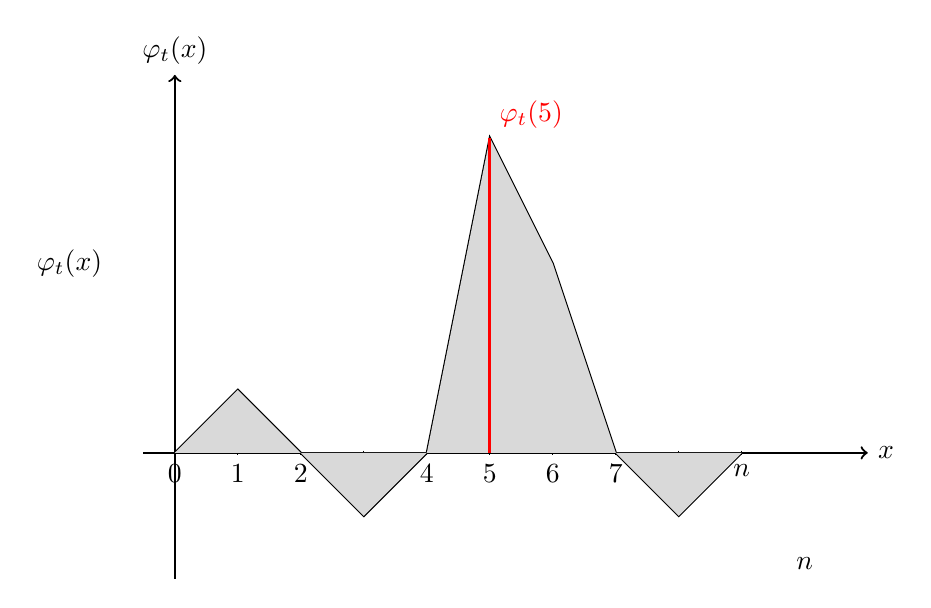
\begin{tikzpicture}[scale=0.8]

% Axes
\draw[->, thick] (-0.5,0) -- (11,0) node[right] {$x$};
\draw[->, thick] (0,-2) -- (0,6) node[above] {$\varphi_t(x)$};

% x-axis ticks and labels
\foreach \x/\label in {0/0, 1/1, 2/2, 3/3, 4/4, 5/5, 6/6, 7/7, 8/8, 9/n}
    \draw (\x cm,1pt) -- (\x cm,-1pt) node[anchor=north] {$\label$};

% Interface line
\coordinate (A) at (0,0);
\coordinate (B) at (1,1);
\coordinate (C) at (2,0);
\coordinate (D) at (3,-1);
\coordinate (E) at (4,0);
\coordinate (F) at (5,5);
\coordinate (G) at (6,3);
\coordinate (H) at (7,0);
\coordinate (I) at (8,-1);
\coordinate (J) at (9,0);

\draw[thick] (A) -- (B) -- (C) -- (D) -- (E) -- (F) -- (G) -- (H) -- (I) -- (J);

% Shading for algebraic volume
\fill[gray!30] (A) -- (B) -- (C) -- (D) -- (E) -- (F) -- (G) -- (H) -- (I) -- (J) -- cycle;

% Red vertical line at x=5
\draw[red, very thick] (5,0) -- (5,5);
\node[red, above right] at (5,5) {$\varphi_t(5)$};

% Annotations
\node at (10, -1.5) [below] {$n$};
\node at (-1, 3) [left] {$\varphi_t(x)$};

\end{tikzpicture}

\end{document}